\documentclass[12pt,a4paper]{article}
\usepackage[utf8]{inputenc}
\usepackage[spanish]{babel}
\usepackage{geometry}
\geometry{margin=2.5cm}
\usepackage{graphicx}
\usepackage{listings}
\usepackage{color}
\usepackage{hyperref}
\usepackage{fancyhdr}
\usepackage{titlesec}
\usepackage{enumitem}

\definecolor{codegreen}{rgb}{0,0.6,0}
\definecolor{codegray}{rgb}{0.5,0.5,0.5}
\definecolor{backcolour}{rgb}{0.95,0.95,0.92}
\definecolor{codepurple}{rgb}{0.58,0,0.82}

\lstdefinestyle{mystyle}{
    backgroundcolor=\color{backcolour},   
    commentstyle=\color{codegreen},
    keywordstyle=\color{blue},
    numberstyle=\tiny\color{codegray},
    stringstyle=\color{codepurple},
    basicstyle=\ttfamily\footnotesize,
    breakatwhitespace=false,         
    breaklines=true,                 
    captionpos=b,                    
    keepspaces=true,                 
    numbers=left,                    
    numbersep=5pt,                  
    showspaces=false,                
    showstringspaces=false,
    showtabs=false,                  
    tabsize=2
}

\lstset{style=mystyle}
\titleformat{\section}{\Large\bfseries}{\thesection.}{1em}{}
\titleformat{\subsection}{\large\bfseries}{\thesubsection.}{1em}{}

\begin{document}

% ====================== PORTADA ======================
\begin{titlepage}
    \centering
    \vspace*{1cm}
    
    
\includegraphics[width=6cm]{imagenes/uam_logo.png}
    
    \vspace{1.5cm}
    
    {\Large \textbf{UNIVERSIDAD AUTÓNOMA METROPOLITANA}} \\
    {\large \textbf{Unidad Cuajimalpa}} \\[0.5cm]
    {\Large \textbf{Sistemas Distribuidos}} \\[2cm]
    
    {\Huge \textbf{Práctica 2: Calculadora Remota Mejorada}} \\[0.5cm]
    {\Large Arquitectura Cliente-Servidor con Frontend y Cliente Intermedio} \\[2cm]
    
    \textbf{Integrantes:} \\[0.8cm]
    Aaron Rodrigo Ramos Reyes\\
    Ismael Valencia Reyes\\
    Fabian Emiliano Castañeda Juvera
    
    \vspace{2cm}
    {\large Ciudad de México, \today}
    
\end{titlepage}

\tableofcontents
\newpage

\section{Introducción}
En esta segunda práctica se mejoró significativamente una aplicación cliente-servidor para realizar operaciones aritméticas básicas (\texttt{+}, \texttt{-}, \texttt{*}, \texttt{/}) de forma distribuida. 

El objetivo principal fue reforzar los conceptos de **arquitectura distribuida**, **separación de responsabilidades** y **comunicación entre procesos**. Se mantiene un servidor robusto en C++, pero se modificó la arquitectura para que el frontend en Python funcione únicamente como interfaz gráfica, delegando toda la lógica de red al cliente en C++ mediante llamadas a subprocess.

Esta nueva estructura permite una mejor modularidad, facilitando el mantenimiento y la escalabilidad del sistema.

\section{Mejoras Realizadas}
Respecto a la práctica anterior, se implementaron las siguientes mejoras:

\begin{itemize}[leftmargin=*]
    \item \textbf{Separación clara de responsabilidades}: El frontend Python ya no se conecta directamente al servidor. Ahora actúa solo como interfaz gráfica.
    \item \textbf{Cliente C++ como capa intermedia}: Se modificó para aceptar parámetros por línea de comandos, permitiendo su ejecución desde Python.
    \item \textbf{Soporte nativo de múltiples clientes}: El servidor maneja concurrentemente múltiples conexiones mediante hilos (\texttt{std::thread}).
    \item \textbf{Mejor experiencia de usuario}: Se agregó un campo editable para la IP del servidor directamente en la interfaz gráfica.
    \item \textbf{Robustez del servidor}: Mejoras en el manejo de buffers, parsing de datos y gestión de errores.
    \item \textbf{Interoperabilidad entre lenguajes}: Uso de \texttt{subprocess} para comunicar Python con el ejecutable C++.
    \item \textbf{Facilidad de conexión}: Cualquier máquina en la misma red puede conectarse usando la IP del servidor.
\end{itemize}

\section{Diagrama de Componentes}

\begin{figure}[h]
    \centering
    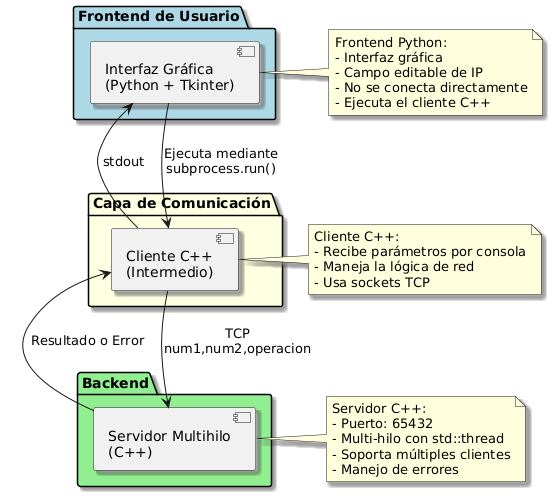
\includegraphics[width=0.85\textwidth]{imagenes/diagrama.png}
    \caption{Diagrama de Componentes de la Calculadora Remota - Práctica 2}
    \label{fig:diagrama}
\end{figure}

\subsection{Explicación de las Relaciones}
El sistema está compuesto por tres componentes principales:

\begin{itemize}
    \item \textbf{Frontend Gráfico (Python)}: Solo interfaz de usuario. No realiza conexiones de red.
    \item \textbf{Cliente C++}: Capa intermedia responsable de toda la comunicación TCP con el servidor.
    \item \textbf{Servidor Multihilo (C++)}: Componente central que procesa las solicitudes.
\end{itemize}

El flujo es: **Python → Cliente C++ (subprocess) → Servidor (TCP)**. La respuesta sigue el camino inverso.

\section{Explicación del Código}

\subsection{Servidor (C++)}
El servidor es el núcleo del sistema. Utiliza sockets TCP y un modelo multi-hilo para atender múltiples clientes simultáneamente.

Las partes clave incluyen:
\begin{itemize}
    \item Configuración del socket con \texttt{SO\_REUSEADDR | SO\_REUSEPORT}.
    \item \texttt{bind()} en todas las interfaces (\texttt{INADDR\_ANY}) en el puerto 65432.
    \item Bucle principal con \texttt{accept()} y creación de hilos para cada cliente.
    \item Función \texttt{atender\_cliente()}: Lee los datos, parsea el formato \texttt{num1,num2,op}, realiza el cálculo y devuelve la respuesta.
    \item Manejo seguro de errores y cierre correcto de sockets.
\end{itemize}

\subsection{Cliente Consola (C++)}
Este componente fue rediseñado para ser invocado desde otros programas. Sus características principales son:
\begin{itemize}
    \item Recepción de parámetros por línea de comandos: IP, num1, num2 y operación.
    \item Creación de socket TCP y conexión al servidor.
    \item Envío del mensaje en formato texto.
    \item Recepción y salida limpia de la respuesta (ideal para capturar con Python).
\end{itemize}

\subsection{Interfaz Gráfica (Python)}
Desarrollada con Tkinter, su rol es exclusivamente visual. Destacan:
\begin{itemize}
    \item Campo editable para la IP del servidor.
    \item Teclado numérico y botones de operación.
    \item Ejecución del cliente C++ mediante \texttt{subprocess.run()} en un hilo separado.
    \item Captura de la salida estándar y manejo de errores amigable.
\end{itemize}

\section{Flujo de Uso}

\subsection{1. Obtener la IP del Servidor}
Ejecutar en la máquina del servidor:
\begin{lstlisting}[language=bash]
ip a | grep inet
\end{lstlisting}
o
\begin{lstlisting}[language=bash]
hostname -I
\end{lstlisting}

\subsection{2. Levantar el Servidor}
\begin{lstlisting}[language=bash]
g++ -std=c++11 -pthread servidor_calculadora.cpp -o servidor
./servidor
\end{lstlisting}

\subsection{3. Compilar el Cliente C++}
\begin{lstlisting}[language=bash]
g++ cliente_calculadora.cpp -o cliente
chmod +x cliente
\end{lstlisting}

\subsection{4. Ejecutar el Frontend Python}
\begin{lstlisting}[language=bash]
python3 frontend_calculadora.py
\end{lstlisting}

\section{Evidencias}

\begin{figure}[h]
    \centering
    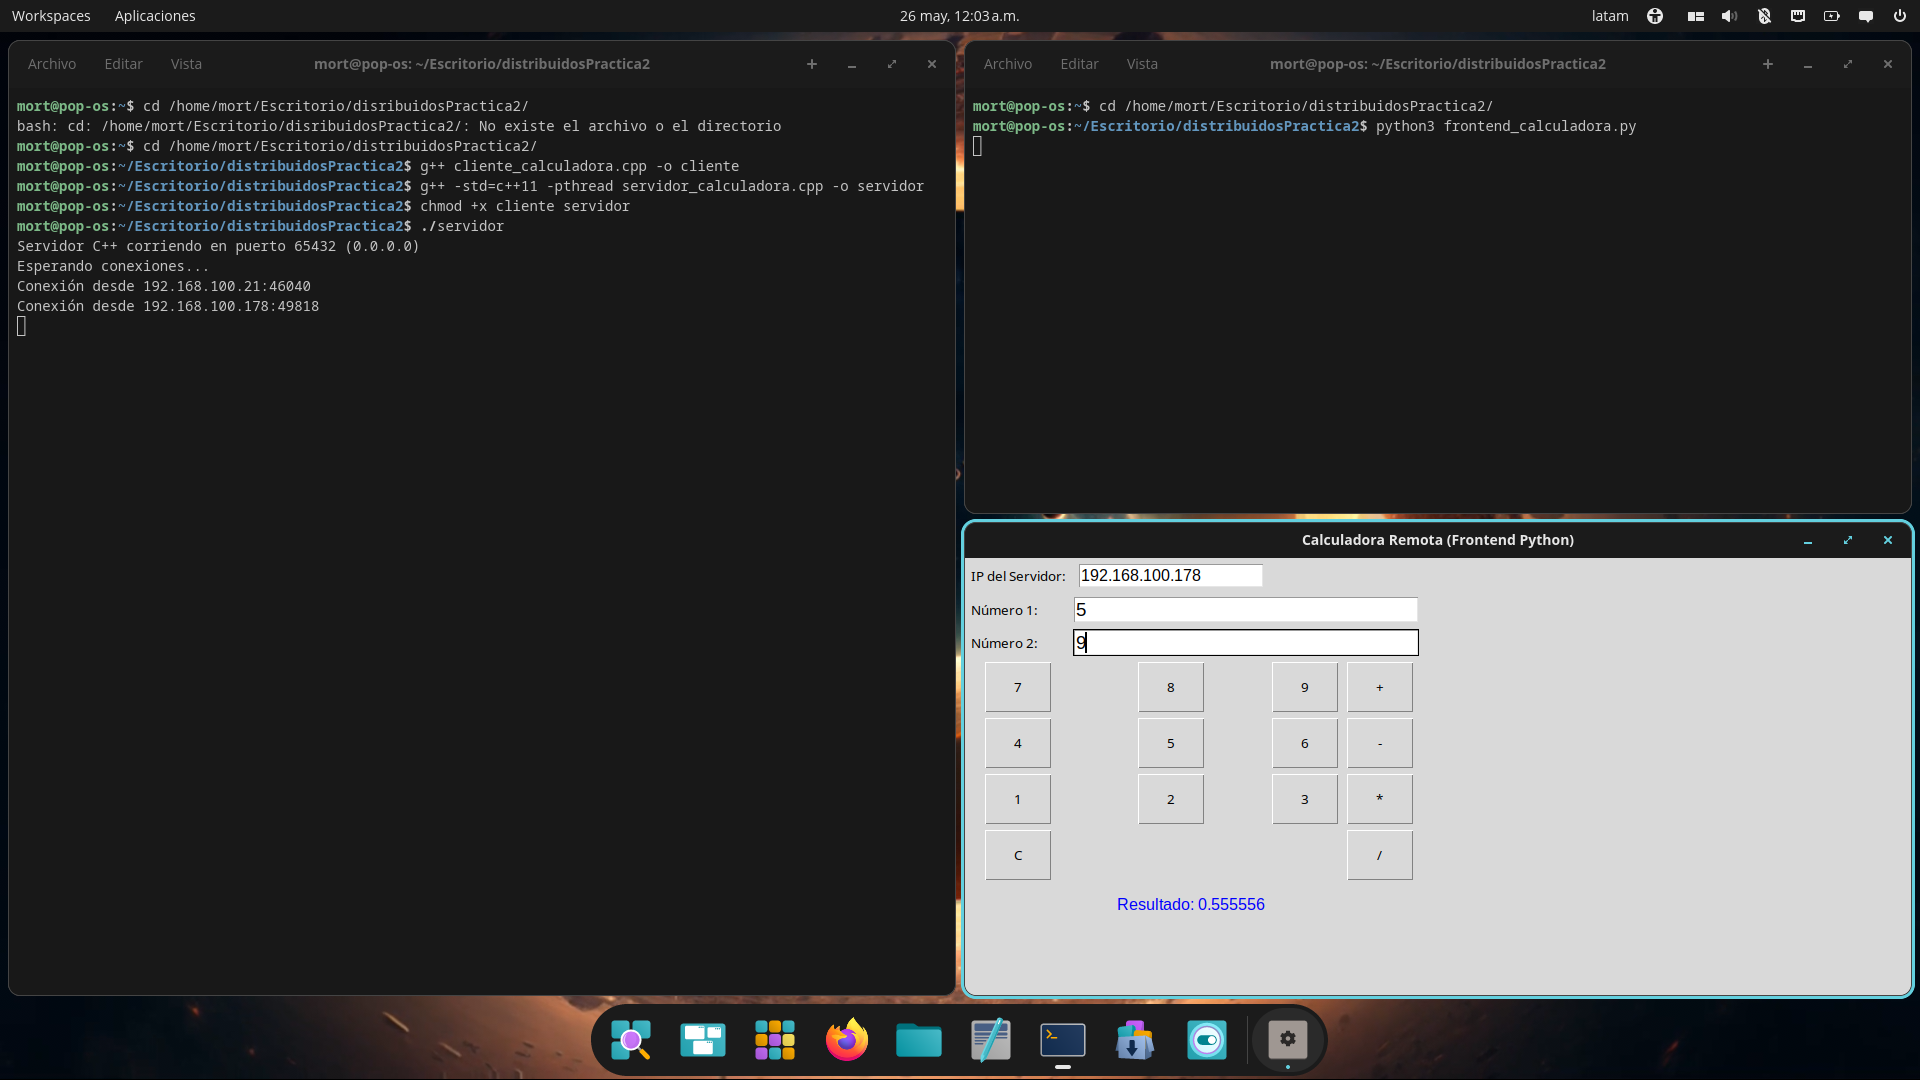
\includegraphics[width=0.95\textwidth]{imagenes/evidencia.png}
    \caption{Evidencia de funcionamiento con múltiples clientes}
    \label{fig:evidencia}
\end{figure}

En esta evidencia se observa:
\begin{itemize}
    \item El servidor ejecutándose y recibiendo conexiones desde dos direcciones IP diferentes.
    \item Un cliente C++ ejecutándose en la misma máquina del servidor.
    \item Otro cliente (a través del frontend Python) conectándose desde una máquina diferente en la misma red.
    \item El correcto procesamiento de operaciones y respuestas.
\end{itemize}

\section{Conclusiones}

Esta práctica permitió consolidar y profundizar los conocimientos en Sistemas Distribuidos. Entre los principales aprendizajes se encuentran:

\begin{itemize}
    \item La importancia de una **buena separación de responsabilidades** en arquitecturas distribuidas.
    \item El uso efectivo de **concurrencia** (hilos) para permitir múltiples clientes simultáneos.
    \item La interoperabilidad entre lenguajes mediante llamadas a procesos (\texttt{subprocess}).
    \item El diseño de protocolos simples pero efectivos de comunicación cliente-servidor.
    \item La relevancia del manejo adecuado de errores y la robustez en entornos de red.
    \item Cómo una interfaz gráfica puede actuar como un "frontend puro" delegando la lógica de red.
\end{itemize}

El sistema desarrollado demuestra de manera práctica cómo construir aplicaciones distribuidas modulares, escalables y mantenibles, cumpliendo con los objetivos de la asignatura.

\end{document}